% ==========================================
% CHAPITRE 3
% ==========================================
\chapter{Méthodologie et moyens mis en œuvre}

\section{Démarche globale et organisation des travaux}

\subsection{Une approche itérative et structurée}

Le projet de migration du datamart Construction a été conduit selon une \textbf{approche itérative et incrémentale}, organisée en cinq phases successives. Ce choix méthodologique s'est imposé naturellement compte tenu des contraintes du projet : un code SAS non documenté à analyser, une architecture cible à concevoir, et un critère de parité fonctionnelle strict à atteindre. Chaque phase s'est appuyée sur les livrables de la phase précédente, garantissant une progression méthodique et tracée.

Ce séquençage reflète un principe fondamental adopté dès le départ : \textbf{analyser et documenter exhaustivement avant d'écrire la première ligne de code}. Cette décision, validée avec le chef de projet, a permis d'éviter les erreurs dues à une mauvaise compréhension de la logique métier, et d'identifier en amont les complexités susceptibles d'impacter les choix architecturaux.

Le tableau \ref{tab:methodologie} présente la vue d'ensemble des cinq phases et leur enchaînement :

\begin{table}[H]
    \centering
    \caption{Vue d'ensemble des cinq phases de la méthodologie de migration}
    \label{tab:methodologie}
    \vspace{0.2cm}
    \begin{tabularx}{\textwidth}{@{}c c c X X@{}}
        \toprule
        \textbf{Phase} & \textbf{Intitulé} & \textbf{Durée} & \textbf{Objectif} & \textbf{Livrable principal} \\
        \midrule
        1 & Analyse et documentation SAS & 2 semaines & Comprendre le code source & Documentation SAS complète \\
        2 & Conception de l'architecture cible & 1 semaine & Définir la structure Python & Architecture médaillon validée \\
        3 & Recensement des règles et datasets & 1 semaine & Inventorier l'exhaustif & 2 fichiers Excel de référence \\
        4 & Implémentation Python & 5 semaines & Développer les pipelines & Code source (3 pipelines) \\
        5 & Validation et tests de parité & 5 semaines & Garantir l'équivalence & Rapports de validation KPI \\
        \bottomrule
    \end{tabularx}
\end{table}

\subsection{Équipe et cadre de travail}

Le projet s'est déroulé au sein d'une équipe restreinte composée du projet et de son chef de projet, Romeo TOHOUN, data scientist et sa responsable hiérarchique Caroline BOUCHON dans le pôle Advanced Data \& Climate. Des points d'avancement hebdomadaires ont permis de valider les choix techniques, de lever les ambiguïtés métier et d'orienter les priorités de développement. La collaboration avec M. Alain VOSS, expert assurance de l'équipe, a été essentielle pour comprendre les mécanismes assurantiels sous-jacents aux règles métier codées en SAS.

\section{Rétro-ingénierie et documentation du code existant}

\subsection{Objectifs et démarche d'analyse}

La phase d'analyse a démarré dans un contexte contraint : un code SAS historique volumineux, non documenté, et techniquement complexe (macros imbriquées, absence de rigueur dans le nommage). L'objectif était de comprendre la logique métier existante avant de concevoir la solution cible.

L'analyse a suivi une méthode \textit{top-down} : étude des fichiers d'orchestration pour le flux global, décryptage des macros métier (cœur des transformations et règles de calcul), puis analyse des fichiers utilitaires. Cette démarche a permis de cartographier de manière exhaustive les sources de données, les transformations, et les tables de sortie pour chaque pipeline, constituant ainsi la base des schémas architecturaux.

\subsection{Livrables produits}

Cette analyse a abouti à la création d'une documentation SAS complète (Voir \hyperlink{annexe.C}{Annexe C}), structurée en un volet synthétique (pour la vision managériale et la pérennité de la connaissance) et un volet technique détaillé décrivant chaque transformation pour guider l'implémentation Python et les futurs tests de parité.

\section{Conception de l'architecture logicielle cible}

\subsection{Évaluation des options architecturales}

Suite à l'analyse du code SAS, deux options d'architecture ont été évaluées et présentées lors d'une réunion de cadrage avec le chef de projet.

La \textbf{réplication à l'identique} aurait consisté à reproduire la structure SAS en Python (un script Python par fichier SAS). Cette option présentait l'avantage d'être simple à valider par comparaison directe, mais elle aurait conservé l'ensemble des défauts de l'architecture monolithique source : séquentialité, couplage fort entre les modules, absence de séparation des responsabilités.

L'\textbf{architecture médaillon complète} (Bronze/Silver/Gold), standard de l'industrie tel que décrit dans le chapitre 2, a été retenue. Cette option nécessitait un effort de développement initial plus important, mais offrait les garanties de qualité, de traçabilité et d'évolutivité requises pour un système en production.

\subsection{Principes de conception retenus}

Quatre principes fondamentaux ont guidé la conception du système Python :

\textbf{Configuration > Code} : les règles métier qui sont susceptibles d'évoluer (filtres, mappings de colonnes, paramètres de seuils) sont externalisées dans des fichiers de configuration JSON et YAML. Cela permet de modifier le comportement du système sans toucher au code, réduisant le risque d'erreurs et simplifiant la maintenance.

\textbf{Modularité} : chaque composant du système remplit une responsabilité unique et bien définie. Les lecteurs de données (\textit{readers}) sont isolés des processeurs métier (\textit{processors}), qui sont eux-mêmes distincts des fonctions de transformation (\textit{utils/transformations}). Cette séparation facilite les tests unitaires et la réutilisation du code entre pipelines.

\textbf{Logging détaillé} : chaque étape de traitement produit des logs structurés indiquant le nombre de lignes en entrée et en sortie, le temps d'exécution et les valeurs clés des indicateurs calculés. Ce niveau de traçabilité est indispensable pour diagnostiquer les éventuelles divergences lors de la validation.

\textbf{Gestion d'erreurs gracieuse} : les enrichissements avec des données optionnelles (référentiels parfois absents) sont traités avec des mécanismes de fallback. Un enrichissement non disponible génère un avertissement dans les logs mais ne bloque pas l'exécution du pipeline.

\subsection{Stack technologique validée}

Les choix technologiques ont été validés en cohérence avec l'infrastructure cloud d'Allianz et les recommandations de l'équipe Data Management :

\begin{table}[H]
    \centering
    \caption{Stack technologique retenue pour l'implémentation Python}
    \label{tab:stack}
    \vspace{0.2cm}
    \begin{tabularx}{\textwidth}{@{}l l X@{}}
        \toprule
        \textbf{Composant} & \textbf{Technologie} & \textbf{Rôle} \\
        \midrule
        Langage & Python 3.11+ & Développement des pipelines \\
        Framework de traitement & PySpark 3.x & Traitement distribué des DataFrames \\
        Format de stockage & Parquet & Optimisation lectures/écritures \\
        Configuration & JSON / YAML & Externalisation des règles métier \\
        Versioning & Git & Traçabilité du code \\
        Environnement de dev & ADP (tout pré‑installé) & Tests et mise au point \\
        \bottomrule
    \end{tabularx}
\end{table}

\section{Recensement des règles de gestion et des données sources}

\subsection{Objectif : tout tracer avant de coder}

Avant de démarrer toute implémentation, un effort systématique de recensement a été conduit pour constituer deux fichiers Excel de référence. Cette étape, inspirée des bonnes pratiques de gestion de projet data, vise à garantir l'exhaustivité de la migration en évitant les oublis qui n'auraient pu être détectés que tardivement.

\subsection{Fichier 1 : inventaire des règles de gestion}

Le premier fichier Excel (\texttt{datamart\_construction\_regle\_de\_gestion.xlsx}) recense l'ensemble des règles métier du datamart, soit \textbf{soixante-douze règles} réparties sur les trois pipelines (Voir \hyperlink{annexe.E}{Annexe E}). Chaque règle est documentée avec un identifiant unique, le pipeline concerné, une description de la règle, la référence précise au code SAS source (fichier et numéro de ligne) et l'implémentation Python correspondante.

Ce fichier a rempli un double rôle : \textbf{checklist d'implémentation} pendant la phase de développement (chaque règle étant cochée après implémentation et validation), et \textbf{base de traçabilité} permettant de vérifier après coup que chaque comportement SAS est bien couvert par le code Python.

\subsection{Fichier 2 : recensement des datasets sources}

La seconde feuille du même fichier inventorie l'ensemble des sources de données du datamart. Au total, \textbf{quarante-cinq groupes de fichiers} (\textit{file groups}) ont été identifiés, couvrant les données mensuelles de portefeuille (fichiers IPF), les données de capitaux et garanties (POLIC\_CU, CAPITXCU), les référentiels métier (segmentation, ISIC, NAF, FFB), et les données de primes (One BI). Pour chaque dataset, le fichier précise la table SAS source, le fichier SAS qui l'utilise, la version (mensuel ou référentiel) et le type (entrée source ou sortie).

Cette dernière information s'est révélée particulièrement précieuse : plusieurs datasets référencés dans le code SAS n'étaient pas disponibles dans le datalake au moment du projet (\texttt{cproduit.csv}, \texttt{prdcap.csv}, \texttt{lob.csv}, ...). Leur identification précoce a permis de les déclarer optionnels en Python et de gérer leur absence de manière gracieuse, évitant des blocages lors de l'exécution.

\section{Implémentation technique des pipelines de données}

\subsection{Structure du projet}

L'arborescence du projet Python suit une organisation modulaire claire, reflétant la séparation des responsabilités adoptée lors de la conception :

\begin{verbatim}
project_baseline/
|-- config/                   # Configuration centralisée
|   |-- reading_config.json   # Paramètres de lecture des sources
|   |-- column_definitions.py # Schémas au format DDL pour Spark
|   |-- config.yml            # Configuration globale de l'application
|   |-- constants.py          # Constantes métier
|   |-- variables.py          # Variables globales du projet
|   `-- transformations/      # Règles métier JSON par pipeline
|-- src/
|   |-- processors/           # Logique métier par pipeline
|   |   |-- capitaux_processors/
|   |   |-- emissions_processors/
|   |   `-- ptf_mvt_processors/
|   |-- orchestrators/        # Orchestration des exécutions
|   `-- reader.py             # Lecture des données Bronze
|-- utils/
|   |-- transformations/      # Fonctions métier (base, operations)
|   |-- loaders/              # Utilitaires de chargement externes
|   |-- helpers.py            # Fonctions génériques (dates, types)
|   |-- processor_helpers.py  # Fonctions d'aide aux processors
|   `-- logger.py             # Logger structuré personnalisé
|-- docs/                     # Documentation technique (configs, workflows)
`-- main.py                   # Point d'entrée principal
\end{verbatim}

Les \textbf{fondations du projet} (module de lecture, helpers, logger, configuration) ont été développées et testées en premier, avant le développement d'un seul pipeline métier. Cette approche a garanti que les briques de base étaient fiables avant de les utiliser dans des contextes métier plus complexes.

\subsection{Ordre d'implémentation et stratégie de développement}

L'ordre d'implémentation des pipelines a été décidé par ordre de complexité décroissante : PTF Mouvements en premier (le plus complexe, impliquant les deux canaux AZ et AZEC, la consolidation, et les enrichissements multiples), puis Capitaux (complexité intermédiaire, avec la logique d'indexation FFB), et enfin Émissions (le plus linéaire, sans consolidation AZ/AZEC).

Le choix d'aborder d'abord le pipeline le plus complexe présente un avantage stratégique majeur : les fonctions utilitaires créées pour PTF Mouvements (extraction des capitaux, calcul des mouvements AFN/RES/PTF, enrichissement ISIC, harmonisation AZ/AZEC) sont directement réutilisables pour les pipelines suivants, réduisant significativement l'effort de développement global.

À l'intérieur de chaque pipeline, une approche \textbf{itérative par transformation} a été systématiquement appliquée : coder une transformation, la tester immédiatement sur un sous-ensemble de données, logger le nombre de lignes en entrée et en sortie, corriger si nécessaire, puis passer à la transformation suivante. Cette discipline a permis de détecter et corriger les erreurs au plus tôt, avant qu'elles ne se propagent et ne deviennent difficiles à tracer.

\subsection{Architecture des processors}

Chaque pipeline est implémenté selon un pattern de classe Python orienté objet, structuré autour de trois méthodes principales : \texttt{read()} pour l'ingestion depuis la couche Bronze, \texttt{transform()} pour l'application des règles métier, et \texttt{write()} pour l'écriture des résultats en couche Silver ou Gold.

L'architecture détaillée des flux de données, illustrée par la figure \ref{fig:python_process_architecture}, permet de visualiser de manière synthétique l'enchaînement des opérations pour les trois pipelines.

\begin{figure}[H]
    \centering
    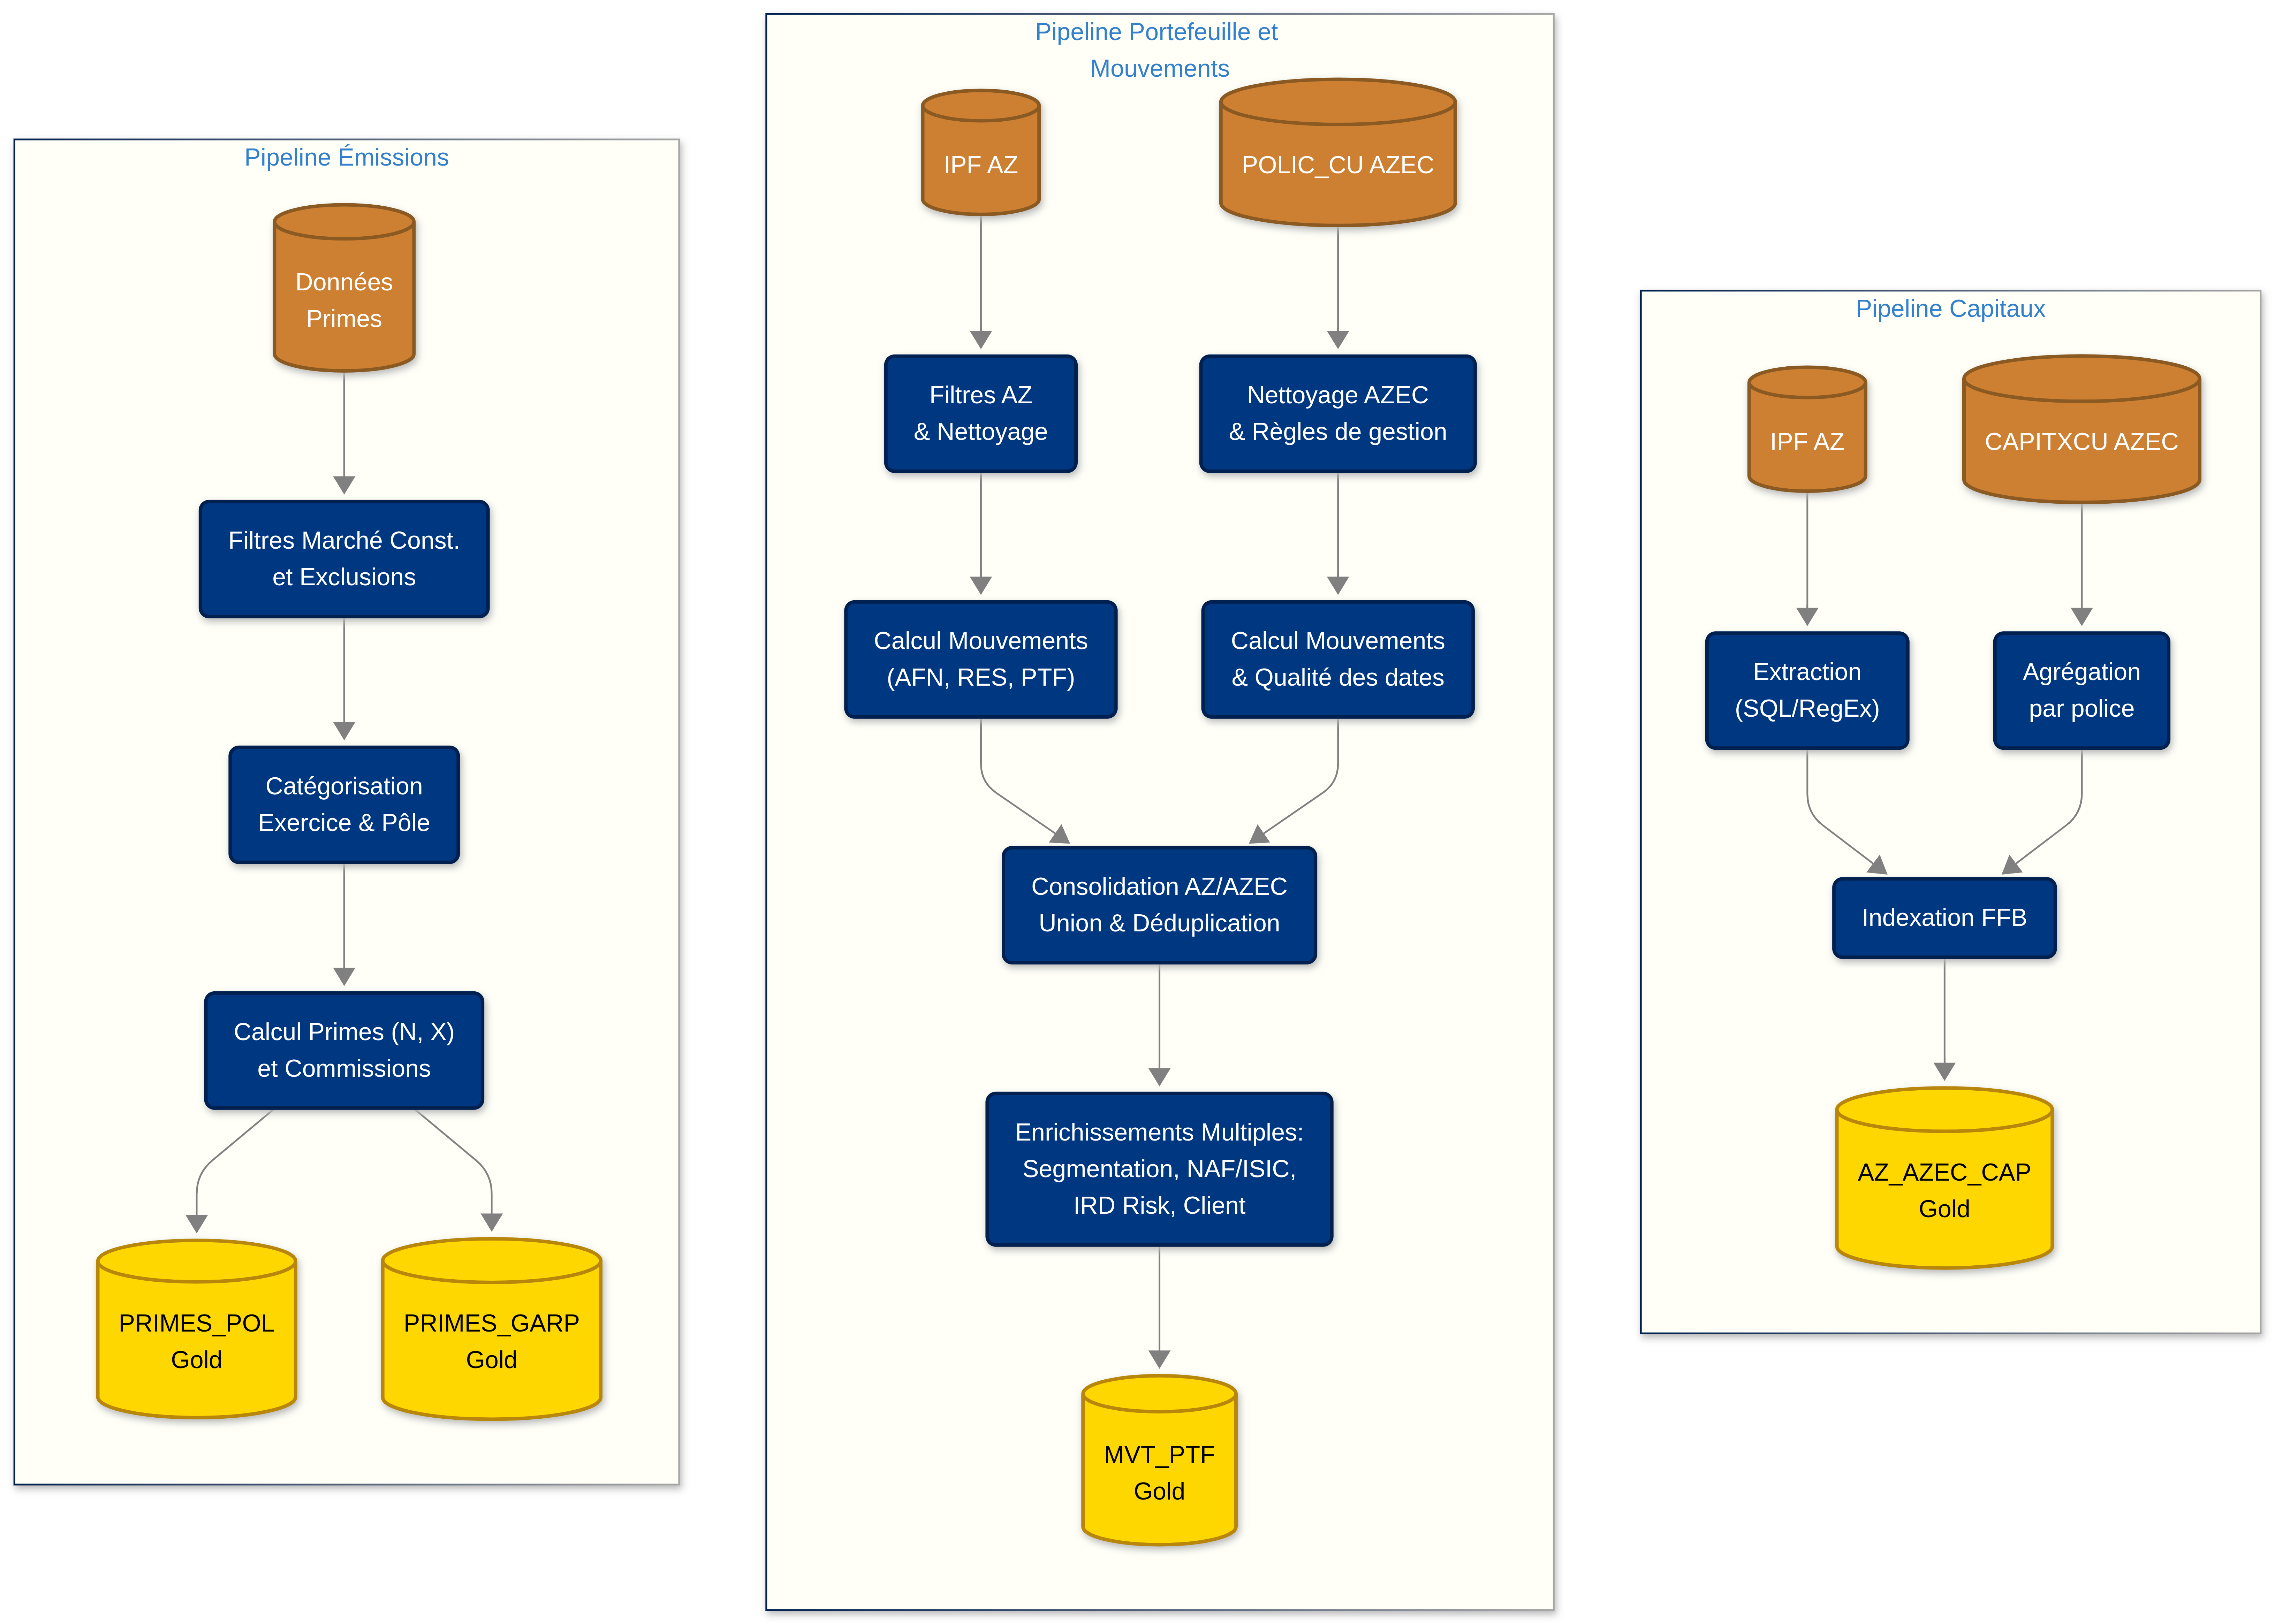
\includegraphics[width=1\textwidth]{schemas/python_process_architecture.png}
    \caption{Architecture fonctionnelle détaillée des trois pipelines PySpark (Capitaux, Mouvements, Émissions), illustrant le cheminement des données de la couche Bronze à Gold.}
    \label{fig:python_process_architecture}
\end{figure}

Cette représentation met en évidence la modularité des traitements, particulièrement visible pour le pipeline \textit{Portefeuille et Mouvements}. Ce dernier nécessite l'exécution d'étapes de nettoyage propres à chaque canal de distribution (AZ et AZEC), suivies d'une consolidation complexe (harmonisation des schémas, union, et enrichissements en cascade via des référentiels externes).

\section{Validation fonctionnelle et stratégie de tests}

\subsection{Stratégie de validation à trois niveaux}

La phase de validation a été organisée selon une approche à trois niveaux de granularité croissante, inspirée des bonnes pratiques de recette fonctionnelle.

La \textbf{validation structurelle} vérifie que les fichiers de sortie Python existent, que leurs schémas contiennent les colonnes attendues avec les types corrects, et que les volumes de données sont cohérents avec les données d'entrée. Ce premier niveau permet de détecter rapidement les erreurs grossières (colonnes manquantes, types incorrects, pipeline incomplet).

La \textbf{validation fonctionnelle} compare les indicateurs agrégés (KPI) entre les sorties SAS et les sorties Python, sur plusieurs visions mensuelles. Les critères retenus sont stricts : un écart inférieur à 0,01\% sur les KPI agrégés (nombre de polices, sommes de primes, totaux de capitaux) est requis pour valider la parité. Cette tolérance quasi nulle garantit que les résultats Python sont exploitables pour les analyses actuarielles et les reportings réglementaires.

La \textbf{validation par échantillonnage} compare champ par champ un échantillon de polices sélectionnées aléatoirement, permettant de détecter des erreurs compensatoires qui pourraient passer inaperçues au niveau des indicateurs agrégés.

\subsection{Défis techniques rencontrés lors de la validation}

La confrontation des résultats Python et SAS a soulevé plusieurs défis techniques ayant nécessité des investigations poussées. L'approche est restée la même : diagnostic via le code SAS, correction en Python, puis rejeu du pipeline pour vérifier la convergence. Voici les principaux problèmes résolus :

\begin{itemize}
    \item \textbf{Disponibilité des données de test :} L'accès aux données de production sur Azure nécessitait des validations de sécurité strictes. Ces délais nous ont souvent obligé à coder "à l'aveugle" en attendant de pouvoir tester sur des données réelles, ce qui rallongeait les cycles de correction.
    \item \textbf{Colonne CDPOLE absente en AZEC :} Lors de la consolidation, Python trouvait moins de polices Courtage (pôle 3) que SAS. L'analyse a montré que SAS forçait l'assignation \texttt{cdpole = "3"} via une macro dédiée. Un simple ajout dans le processor AZEC a rétabli la parité.
    \item \textbf{Formats de dates hétérogènes (\texttt{dtechann}) :} La date d'échéance annuelle mélangeait plusieurs formats historiques (MMJJ, MMJJAA, formats complets). Plutôt que d'utiliser un type Date natif qui plantait sur les anomalies, nous avions reproduit la logique SAS en traitant la colonne comme du texte pour extraire et recombiner les caractères, couvrant ainsi 100\% des cas.
    \item \textbf{Dates au format SAS datetime (IRD) :} Les tables IRD Risk contenaient des chaînes complexes (ex: \texttt{'14MAY1991:00:00:00'}) incomprises par PySpark, produisant des valeurs nulles silencieuses. Nous avions dû développer un helper \texttt{parse\_sas\_datetime()} pour extraire et convertir spécifiquement la partie date.
    \item \textbf{Configurations JSON capricieuses :} Pour le filtrage des Émissions métier, nous avions organisé un JSON lisible avec descriptions et valeurs. Cependant, utiliser ce dictionnaire directement dans un \texttt{isin()} PySpark déclenchait une erreur. Nous avions dû extraire explicitement la liste des valeurs en Python pour que Spark l'accepte sans broncher.
    \item \textbf{Harmonisation AZ vs AZEC :} Les deux canaux avaient des noms de colonnes différents (ex: \texttt{POLICE} vs \texttt{NOPOL}). Pour éviter un code rigide rempli de \texttt{withColumnRenamed}, nous avions externalisé tout le mapping dans un JSON dédié, permettant de renommer les colonnes dynamiquement avant l'union.
\end{itemize}

\section{Environnement de développement et livrables}

\subsection{Environnement de développement}

Le développement a été réalisé dans un environnement cloud ADP (Allianz Data platform) qui est automatiquement connecté à azure via un token, permettant de tester l'intégralité des pipelines sans nécessiter de connexion ardure à l'infrastructure cloud Azure. Cette autonomie a facilité le cycle de développement itératif, réduisant les temps de feedback entre la modification et le test. La migration vers Azure Databricks est prévue pour la phase de déploiement en production, postérieure à la période du mission.

La gestion du code source a été assurée via Git, avec un dépôt versionné permettant de tracer l'ensemble des modifications et de revenir en cas de régression. Cette pratique, absente du système SAS source, constitue l'une des améliorations fondamentales apportées par la migration.

\enlargethispage{2cm} % Ajuste la valeur (1cm, 2cm, etc.) pour gagner de la place en bas
\subsection{Synthèse des livrables produits}

L'ensemble des travaux réalisés au cours du mission a abouti à quatre catégories principales de livrables :

\vspace{0.3cm}
\noindent\fbox{
    \begin{minipage}{\textwidth}
        \vspace{0.2cm}
        \begin{center}
            {\large \textbf{Synthèse des livrables produits lors du mission}}
        \end{center}
        \vspace{0.4em}

        \textbf{1. Documentation Fonctionnelle \& Analyse SAS}
        \begin{itemize}[leftmargin=1.2em]
            \item \texttt{general\_sas\_architecture.drawio} — \emph{Schéma de l'architecture générale SAS (datamart).}
            \item \texttt{sas\_detail\_flow\_architecture.drawio} — \emph{Architecture détaillée des trois workflows SAS.}
            \item \texttt{documentation\_datamart\_construction\_sas\_26112025.pptx} — \emph{Présentation complète incluant logique métier, traitements et organisation.}
            \item \texttt{Architecture\_Générale\_doc\_sas.docx} — \emph{Documentation générale du code SAS et de sa structure.}
            \item \texttt{Analyse de l'Architecture SAS Construction.md} — \emph{Documentation détaillée au format Markdown.}
        \end{itemize}

        \textbf{2. Documentation Métier (Règles \& Datasets)}
        \begin{itemize}[leftmargin=1.2em]
            \item \texttt{datamart\_construction\_regle\_de\_gestion.xlsx} — \emph{72 règles métier documentées et 45 datasets inventoriés.}
        \end{itemize}

        \textbf{3. Développement Python}
        \begin{itemize}[leftmargin=1.2em]
            \item \texttt{python\_architecture.excalidraw} — \emph{Architecture Medallion (Bronze $\to$ Silver $\to$ Gold) détaillant modules et pipelines.}
            \item \emph{Pipelines Python alignés avec les workflows SAS (dépôt GitHub interne Allianz).}
        \end{itemize}

        \textbf{4. Assurance Qualité (QA)}
        \begin{itemize}[leftmargin=1.2em]
            \item \texttt{kpis\_results.xlsx} — \emph{Comparaison des résultats SAS vs Python (KPI, écarts et performances).}
        \end{itemize}
        \vspace{0.2cm}
    \end{minipage}
}
\vspace{0.3cm}
